\documentclass{../tex_import/ETHuebung_english}

\usepackage{../tex_import/exercise_ml}

\input{../tex_import/definitions} %our customized .tex macros

\begin{document}


\makeheader{3, Sept 26, 2024}{Least Squares, Ridge Regression, and Overfitting}

\paragraph{Goals.}
The goal of this exercise is to
\begin{itemize}
\item Implement and debug least-squares.
\item Implement, debug, and visualize basis function models.
\item Understand overfitting.
\item Implement ridge regression.
\end{itemize}

\paragraph{Setup, data, and sample code.}
Obtain the folder {\tt labs/ex03} of the course GitHub repository
\begin{center}
\href{https://github.com/epfml/ML\_course/tree/main/labs/ex03}{github.com/epfml/ML\_course}
\end{center}
We will continue to use the dataset {\tt height\_weight\_genders.csv}
as well as a new dataset {\tt dataEx3.csv} in this exercise.
We have provided sample code that already contains useful snippets of code
required for this exercise.
% The code structures are as follow:
% \begin{itemize}
% \item build\_polynomial.py
% \item cost.py - from exercise02
% \item helpers.py
% \item ridge\_regression.py
% \item split\_data.py
% \end{itemize}

You will be working in the notebook {\tt ex03.ipynb} for the exercises of this week,
by filling in the corresponding functions in the provided template code.

\section{Least Squares and Linear Basis Functions Models}
\subsection{Least squares}

\Exercise{1}{
\begin{itemize}
\item
Fill in the notebook function {\tt least\_squares(y, tx)}
% \footnote{the corresponding function is located in ``least\_squares.py''.}
which implements the solution of the normal equations as discussed in the class.  This
function should return the optimal weights and the mean-squared error. \\
Hint: You should not try to solve a linear system $Ax=b$ by using the \texttt{numpy.linalg.inv} function.

\item To debug your code, you can use the output of the last exercise.
Run gradient descent or grid search on the height-weight data from the last exercise,
and make sure you get a similar resulting $\wv$ vector using all three methods.
% \item Try various versions of least-square implementations given in the lecture notes.
% They must all give the same answer.
\end{itemize}

This is a useful method to debug your code,
i.e. first implementing a simple method and then using it to check more complicated methods.
If you have not finished Exercise 2, please first finish implementing the grid search method.
If you are lagging behind, do not worry. You will get the opportunity to catch up later,
but it is important that you eventually take time to finish previous exercises.
}

\subsection{Least squares with a linear basis function model}
We will now implement and visualize a basis function model for the data {\tt dataEx3.csv}.
\newline

As explained in the class, linear regression might not be directly suitable for nonlinear data.
We will use polynomial basis functions to fit nonlinear data.
\begin{align}
\phi_j(x) := x^j
\end{align}
As we have seen in the lecture notes, the technique of feature expansion by the linear basis function model does allow us to still use linear regression techniques, to fit nonlinear data (recall that in our first simple setting, we assume that each input point is just one real value).
As a result, we will be able to fit the data using different degrees of polynomials,
e.g. a degree two polynomial (which is a linear combination of $1$, $x$ and $x^2$),
or a degree three polynomial (which is a linear combination of $1$, $x$, $x^2$ and $x^3$), etc..
Higher degree polynomials are more expensive to compute and to fit, but can capture finer details in the data, which results in more expressive models.
Think about the pros and cons of choosing a very high or very low degree.
\newline

To measure the fit of our model, we will use a cost function called the Root-Mean-Square-Error (RMSE).
It is related to MSE as follows:
\begin{align}
\text{RMSE}(\wv) := \sqrt{2\cdot\text{MSE}(\wv)}
\end{align}

The magnitude of MSE can be difficult to interpret since it involves a square,
while RMSE provides a more interpretable measure on the same scale as the error of one point.
There are better measures in terms of statistical properties, like $R^2$, but we don't need these for now. See the book
``Introduction to Statistical learning'' if you're interested in more details.
\newline

Let us now implement polynomial regression, using the technique of linear basis functions, and visualize the predictions.

\Exercise{2}{
The goal of this exercise is to plot the data along with predictions using polynomial regression.
Your goal is to find a good $\wv$ using polynomial regression, when using polynomials of  degrees 1, 3, 7, and 12 respectively.
You might want to reuse the function from the previous exercise to calculate the RMSE.
\begin{itemize}
\item
Fill in the notebook function {\tt build\_poly(x, degree)}.  The input of this function is the vector of the data examples $x_n\in \R$ for $1\le n \le N$. As an output, the function must return the extended feature matrix 
\[
\tvPhi := \begin{bmatrix}\phiv(x_1)\\[-1mm]..\\ \phiv(x_n)\\[-1mm]..\\ \phiv(x_N)\end{bmatrix}
\text{ ~ where ~ } \phiv(x_n) := [1,\, x_n,\, x_n^2,\, x_n^3,\, \ldots,\, x_n^{\text{degree}}]
\]
that is the matrix formed by applying the polynomial basis functions to all input data, for the degree of $j=0$ up to $j=${\tt degree}.

When finished, you must COPY your implementation to the separate file {\tt build\_polynomial.py} for the plot function to work.

\item Fill in the notebook function {\tt polynomial\_regression()}. If the code runs successfully, you will see the data and the fit.
You will clearly see why linear regression is not a good fit,
while polynomial regression produces a better fit.

\item You can see that RMSE decreases as we increase the degree of the polynomial.
Does it mean that the fit gets better as we increase the degree?
Which fit is the best in your view?
\end{itemize}
}

\section{Evaluating Model Prediction Performance}
The answer to the last question should be clear if you followed the lecture.
If not, discuss with others and clarify.
\newline

In practice, it matters that predictions are good for unseen examples, not only for training examples.
To simulate the reality, we will now split our dataset into two parts: \textit{training} and \textit{testing}.
We will fit the data using training data and compute RMSE on both test and training data.

\Exercise{3}{
The notebook function {\tt train\_test\_split\_demo()} is supposed to
show the train and test splits for various polynomial degrees.
\begin{itemize}
\item To split the data,
please fill in the notebook function {\tt split\_data(x, y, ratio, ...)}.
Do you think that the order of samples is important when doing the split?
\item Fill in the notebook function {\tt train\_test\_split\_demo()}.
If the code runs successfully, you will see RMSE values printed for degrees 3, 7, and 12.
For each degree, there are again three RMSE values
which correspond to the following three splits of the data.

\begin{itemize}
\item 90\% training, 10\% testing
\item 50\% training, 50\% testing
\item 10\% training, 90\% testing
\end{itemize}

\item Look at the training and test RMSE for degree 3.
Does this make sense? Why?
\item Now look at RMSE for the other two degrees.
Do these make sense? Why? 
\item Which split is better? Why?

\item The test RMSE for degree 12 is ridiculously high for the split 10\%-90\%.
Why do you think this is the case?
\item \textbf{BONUS:} Imagine you have 5000 samples instead of 50.
Which split might be better in that situation?
\end{itemize}
}

\section{Ridge Regression}
The previous exercise shows overfitting when using complex models.
Let us now correct it using Ridge Regression, defined as
\[
\min_{\wv} \quad \frac{1}{2N} \sum_{n=1}^N \big[y_n - \xv_n^\top \wv \big]^2 \ + \ 
\lambda \|\wv\|_2^2
\]

\begin{itemize}
\item Fill in the notebook function {\tt ridge\_regression()}.
% \footnote{the corresponding file is located in {\tt ridge\_regression.py}.}
You can debug your code by setting $\lambda=0$.
This should essentially give the same answer as least-squares code.
You can also check that for large value of lambda, RMSE should be really bad.
\item Play with the demo {\tt ridge\_regression\_demo()}
by choosing a split of 50\%-50\% and plot train and test errors vs $\lambda$ for polynomial degree 7.
You should get a similar plot as Figure~\ref{fig:ridge_regression}.
\end{itemize}

\begin{figure}[!htp]
\centering
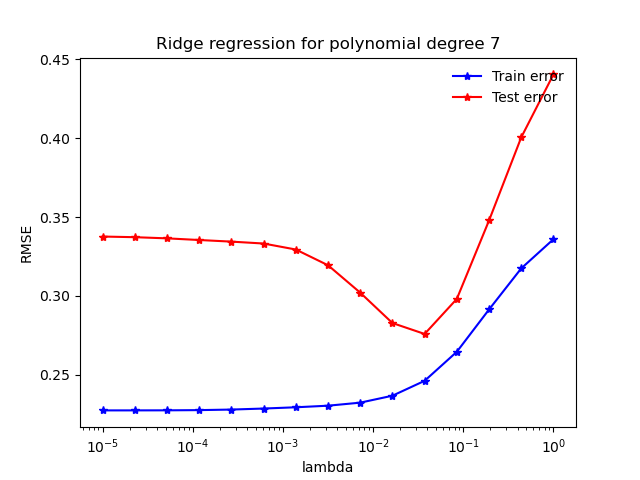
\includegraphics[width=11cm, height=7cm]{solution/ridge_regression.png}\vspace{-1em}
\caption{Ridge Regression Demo.}
\label{fig:ridge_regression}
\end{figure}


\newpage
\section*{Theory Exercises}

\begin{enumerate}
	\item Warm-Up

  \begin{enumerate}
	  \item Show that the sum of two convex functions is convex.

    Hint: use the definition of convexity,
		\[
		f : X \rightarrow \R
		\text{ is convex }
		\ \Leftrightarrow\
		\forall \xv, \yv \in X, \forall \lambda \in [0,1] :
		f(\lambda \xv + (1-\lambda)\yv) \leq \lambda f(\xv) + (1-\lambda)f(\yv).
		\]

  	\item How do you solve the linear system $\mathbf{A}\xv = \bv$? When is it not possible, and why?

  		Hint: \href{https://en.wikipedia.org/wiki/Invertible_matrix}{\textcolor{blue}{Invertible matrix}}
  	\item What is the computational complexity of
	\begin{itemize}
	\item Grid search?
	\item (one step of) Gradient Descent for linear regression with MSE cost?
	\item (one step of) Stochastic Gradient Descent for linear regression with MSE cost?
	\end{itemize}
    	If needed, refresh your memory of the \href{https://en.wikipedia.org/wiki/Computational_complexity_of_mathematical_operations\#Matrix_algebra}{\textcolor{blue}{complexity of algebraic operations}}.
		\item Consider a problem with two input variables, $\xv=(x_1,x_2)$, and one output variable $y$.
			Given the two samples below, find the coefficients $\wv=(w_1,w_2)$ of the linear relationship $\xv^\top\wv = w_1 x_1 + w_2 x_2 = y$.

			\begin{center}
				\begin{tabular}{r|rrr}
					          & $x_1$ & $x_2$ &  $y$	\\
					\hline
					Sample 1  &   400 &  -201 &  200	\\
					Sample 2  &  -800 &   401 & -200	\\
				\end{tabular}
			\end{center}

			Do the exercise again, but with a slight change in the inputs: $x_1$ for sample 1 is now 401 instead of 400

			\begin{center}
				\begin{tabular}{r|rrr}
					          & $x_1$ & $x_2$ &  $y$	\\
					\hline
					Sample 1  &   401 &  -201 &  200	\\
					Sample 2  &  -800 &   401 & -200	\\
				\end{tabular}
			\end{center}

			Compare the resulting $\wv=(w_1,w_2)$ for both cases. Familiarize yourself with the concept of \href{https://en.wikipedia.org/wiki/Condition_number}{\textcolor{blue}{condition number}} as a way to diagnose ill-conditionning. You can find condition number calculators online or use \href{http://docs.scipy.org/doc/numpy-1.10.1/reference/generated/numpy.linalg.cond.html}{\textcolor{blue}{\texttt{numpy.linalg.cond}}}).
  \end{enumerate}

	\item Cost functions

	A cost function defines how you evaluate a solution, and you might have different requirements depending on the problem.
	Using the MSE, if a your model makes an error of 5 on a sample, you add 25/2 to the cost of your model, regardless of the target.
	You might want to penalize this differently if you care about the relative error;
	an output of 1005 when 1000 was expected might be OK, but mistaking a 6 for a 1 might not.
	In this case, you can use a function that takes the relative error of the target $y_n$ into account, like this one:
	\[
	\costfunc_n(f(\xv_n,\wv), y_n) := \frac{(f(\xv_n,\wv) - y_n)^2}{{y_n}^2 + \epsilon}.
	\]
	Where $f$ is the model and $\epsilon$ is a small constant to avoid divisions by zero. Note that we have defined the cost function per example here. You can imagine the total cost function being defined as $\costfunc:=\frac1N\sum_{n=1}^N\costfunc_n$.
  \begin{enumerate}
	  \item Try the function on some [prediction, target] pairs, or plot it, to see how it behaves (by hand or using Python or the wolfram alpha website, no need to code)
  	\item Compute its gradient, assuming a standard linear regression $f(\xv_n, \wv) := \xv_n^\top \wv$
  	\item How would you implement the gradient? Again, no need to code - try to find a formula using standard matrix operations, along with element-wise multiplication and summation/product over columns/rows.
  	\item How sensitive is this function to outliers? Compare two cases: the target is 1, but in one case our model assigns it 10, and in the other 100. (e.g. with $\varepsilon = 1$) How does the error changes? Compare with the following cost function, for the $n$ data example:
  	\[	\costfunc'_n(f(\xv_n,\wv), y_n) := \big(\log(f(\xv_n,\wv)+1) - \log(y_n + 1)\big)^2.	\]
  	Note: The higher the error on a sample is, relative to the other samples, the more your model will try to fit this sample.
  \end{enumerate}
\end{enumerate}

\end{document}
